\sffamily
\chapter{Motivation und Aufgabenstellung}\label{cha:Motivation}

%%%%%%%%%%%%%%%%%%%%%%%%%%%%%%%%%%%%%%%%%%%%%%%%%%%%%%%%%%%%%%%%
% Motivation
%%%%%%%%%%%%%%%%%%%%%%%%%%%%%%%%%%%%%%%%%%%%%%%%%%%%%%%%%%%%%%%%
\section{Motivation}
\blindtext

%%%%%%%%%%%%%%%%%%%%%%%%%%%%%%%%%%%%%%%%%%%%%%%%%%%%%%%%%%%%%%%%
% Aufgabenstellung
%%%%%%%%%%%%%%%%%%%%%%%%%%%%%%%%%%%%%%%%%%%%%%%%%%%%%%%%%%%%%%%%
\section{Aufgabenstellung}
\blindtext
Mehr zu \acp{URI} kann der nachfolgenden Abbildung \ref{fig:uri} entnommen werden. Alles weitere Anhang \ref{anh:index}.

\begin{figure}[H]
	\centering
	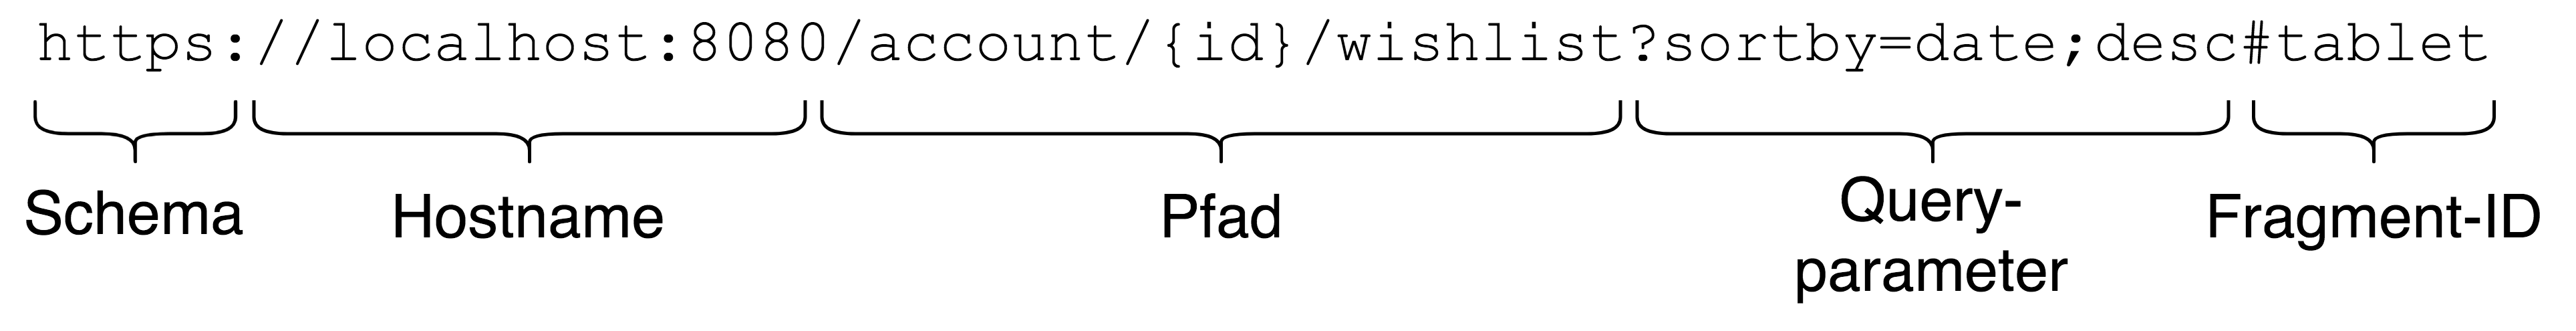
\includegraphics[scale=0.1]{uri-aufbau}
	\caption{Grundprinzip \acs{URI}}
	\label{fig:uri}
\end{figure}

\blindtext
